\documentclass{article}
\usepackage[english]{babel}
\usepackage[latin1]{inputenc}
\usepackage[T1]{fontenc}
\usepackage{listings}
\usepackage{color}
 \usepackage{graphicx}
\usepackage{mathtools}
\usepackage{hyperref}
\definecolor{codegreen}{rgb}{0,0.6,0}
\definecolor{codegray}{rgb}{0.5,0.5,0.5}
\definecolor{codepurple}{rgb}{0.58,0,0.82}
\definecolor{backcolour}{rgb}{0.95,0.95,0.92}

\lstdefinestyle{mystyle}{
    backgroundcolor=\color{backcolour},   
    commentstyle=\color{codegreen},
    keywordstyle=\color{magenta},
    numberstyle=\tiny\color{codegray},
    stringstyle=\color{codepurple},
    basicstyle=\footnotesize,
    breakatwhitespace=false,         
    breaklines=true,                 
    captionpos=b,                    
    keepspaces=true,                 
    numbers=left,                    
    numbersep=5pt,                  
    showspaces=false,                
    showstringspaces=false,
    showtabs=false,                  
    tabsize=2
}
 \lstset{style=mystyle}

\begin{document}
\title{Study on co-occurring critics}
\author{Ricardo Martins-Julien Le Van Suu}
\date\today
\maketitle
\section{Introduction}
A program which produces intelligent and non redundant critics should always be preferred. Having that kind of program can make a lot of difference in terms of productivity, cost efficiency,... 
In a first part we will study the issues in a "dumb" way : that's say counting the critics and calculate the distance.
For that, we will use two representatives packages. We will not put irrelevant issues, as theses should be always removed. The study will be done by method as this is more relevant for Checkstyle. In every package, we pick only two classes as there are big classes which counts more than 500 errors. \\
For finishing, we will provide some high levels critics (For example sometimes some co occurring patterns may be great) and suggest a way to improve the CkeckStyle program. The semi automatic excel file is available here : \url{https://github.com/bigjulien/mmreport}

\section{Study on the co occurring critics}

\subsection{Sorting the results : Statistics method} 
For finding the anomalies, we rely on some intervals : 

\begin{itemize}

\item The results in the range $[0 ; m-\sigma]$ ($\sigma$ the standard deviation and m the mean of the distances between one rules and all others, except itself) will be highlighted in green with red font(baucause if there is a correlation, it's a strong one). \\
The reason is a value outside $[m-\sigma ; m+\sigma]$ is , in stats, a "abnormal" value. \\ Of course, we don't take the 0 coming from the C(n) compared to C(n) rule into account. \\ 

\item The values between $[m-\sigma;0.9]$ will be also highlighted in green. Why 0.9 ? It is recommended in the paper, and furthermore, it seems to don't miss something (a lot of values are = 0.9). Actually, if we would want to be sure to have max precision, we would just do all the pairs of issues(which correspond to a interval of [0 - 1]. \\ However, the following results gives us also great information about the strength of the correlations. \\
It's always a trade off between precision and fastening of the process. \\

All the results between 0 and 0.9 will be studied \\

\item the values which are founded to be interesting patterns will be in bold.

\end{itemize}

\subsection{Results} 
\subsubsection{First package: Root package }
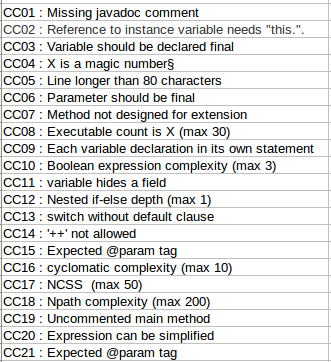
\includegraphics[scale=0.5]{names00.png}\\ \\
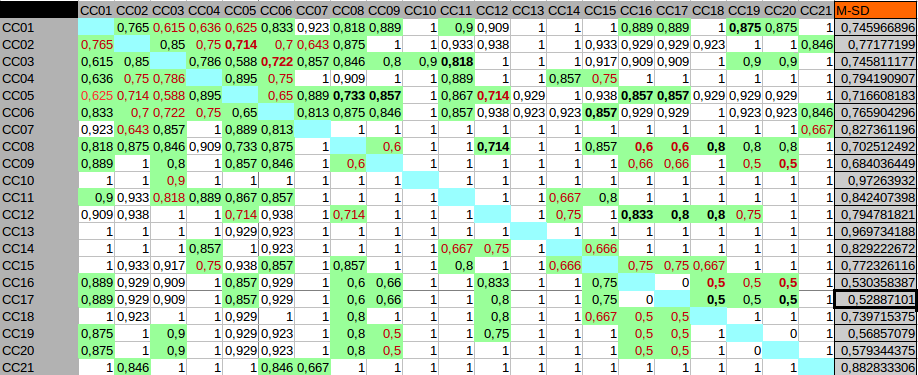
\includegraphics[scale=0.5]{00.png} \\
There is a sight error because Excepted @Param tag appears two times, but it doesn't influence final results.

\subsubsection{Second package : Graphic2D}
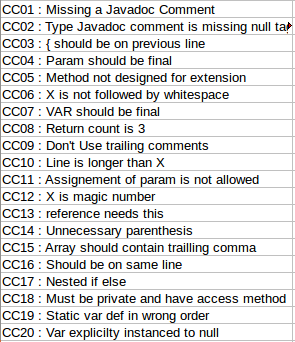
\includegraphics[scale=0.5]{names01.png} \\ \\
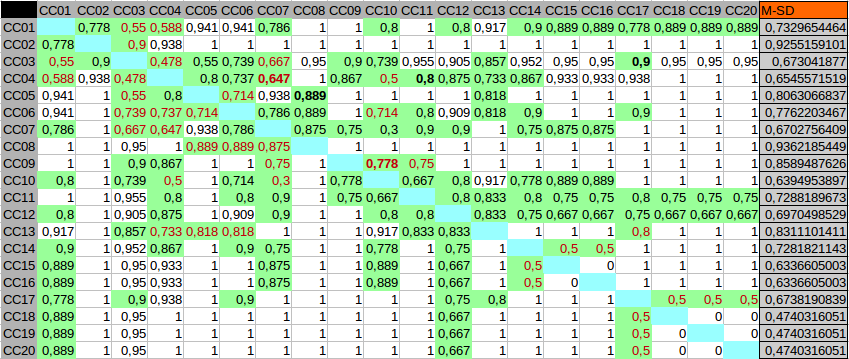
\includegraphics[scale=0.5]{01.png} \\

The results are perhaps a lot disturbing because of some 0 outside the diagonal .\\

The explanation is that the rarer errors in terms of occurrences are in the bottom of the table (because we found them after the others, this is logical in a probability point of view). Theses errors are likely to have strange values, because of the few cases they are implied in. \\
However, we won't discuss them (as advised in the code critics documents) because there is almost no chance to discover an interesting pattern.


\section{Classification on those critics : Package 1}


\subsection{Redundant Critics}
\paragraph{CC16,CC17 - CC18 }
 "Cyclomatic" - "NCSS" \& "NPath" \\
The two complexity issues seems to be correlated to the NPath but not correlated together. Why not just delete the NPath, which overlaps those two ?

\subsection{Overlap Requires Splitting}
\paragraph{CC09  - CC20}
"Each var declaration in own statement" - " Expression can be simplified" \\
We can split the" expression can be simplified" in : cc09 :"each var declaration in own statement" and "too much or/and in the expression" 

\subsection{Overlap Requires Merging}
\paragraph{CC07 - CC16,17,18}
"Executable count is X" -  "Complexities"\\
Of course if there is a lot of executable statement the complexity is bad. As this is calculated in the complexity, we should fusion in a rule "X complexity is too high because of X executable statements) 





\subsection{Same niche}
\paragraph{CC01 - CC19} 
 "Missing Javadoc Comment" - "Uncommented Main method" \\
Theses two are speaking of the same entity : comments so it's likely that the developer which don't judge useful to comment his main don't judge useful to comment the overall class also.
\paragraph{CC03 - CC11} 
"Variable should be declared Final" -  "Variable hides a field" \\
These issues are about variables.

\paragraph{CC06 - CC15} 
"Parameter should be final" - "Missing @parameter" \\
Trivial

\subsection{Almost subset}
\paragraph{CC02 - CC05} 
"Needs this" - "Line longer than 80 characters"
As there is a lot of very long class names in this project, using the name class instead of this will case an increase of the number of characters
\paragraph{CC05 - CC09} 
 "Line is longer than" -  "Each variable declaration in its own statement" \\
If a variable is declared like that it will likely increase the number of characters.
\paragraph{CC05 - CC12} 
"Line is longer than" -  "nested if depth"\\
The algorithm is counting tabulations and spaces, we can see when there is a lot of indentation due to ifs, it will also produce a too long line issue.


\subsection{High level critics}
\paragraph{CC03  - CC06} 
"Var should be declared final" - "Parameter should be declared final" \\
This is almost trivial : When the developer wants to make calculations, rename variable in the body of the method, we will not "cast" the parameter into a final one.
\paragraph{CC05  - CC08} 
"Line longer than" - "Exec count is X"  \\
This means than the code is probably too complex. Theses two alerts together are giving us a hint to the code complexity, which is great.
\paragraph{CC05:  - CC16,17:  }
"Line longer than" - "Complexity matters" \\
Same like above.

\paragraph{CC12 - CC16,17,18}
"Nested if depth" - "Complexities" \\
Excepted because if there is a lot of nested ifs this increase the complexity. We should not recommend to merge them because it gives us additional information about the source of the complexity.



\subsection{Accidental Correlation}
Just one example will be putted there, as this is all the relations CC(i)-CC(j) we haven't mentioned before. \\ We won't highlight this kind of issues in excel as they are not interesting.
\paragraph{CC01 - CC03}
"Missing Javadoc Comment" -  " \} Should be on previous line" \\

\subsection{Noisy correlation}
We won't highlight in the excel file this kind of issues.
\paragraph{CC04 - CC05,06}
 "Param should be final" -  "Method not designed for extension"\&"Line is longer than"


\section{Classification on those critics : Package 2}
We will only put there new correlations founded.

\subsection{Almost subset}
\paragraph{CC04 - CC11}
 "Param should be final" - "Assignement of param is not allowed"  \\
If we resolve the first we resolve also the second. Actually, we don't recommend to delete one of those two.

\paragraph{CC09 - CC10}
 "Trailing comments" - "Line is longer than" \\
If there is comments the line will be likely longer ...

\subsection{High level critics}
\paragraph{CC03 - CC17} 
"\{ Should be on previous line" -  "Nested if else" \\
In if there is likely a \{ so theses two are correlated, but it's actually good.

\paragraph{CC05 - CC08} 
 "Method not designed for extension" - "Return count is 3"
This is actually giving us a hint of why this return count is hight : The method is not designed to be extended. Perhaps we should re factor and do inheritance. This is two good critics.


\section{Improvements and comments on co occurring critics} 
We can see that most of the problematic correlations are overlaps and subsets. \\We would recommend to split into more smaller part the problems and so having accuracy and not any overlap or subset. \\


\section{Conclusion}
For a measure program developer, the just middle between be too fined or too coarse is very  hard to find. This is also normal to find correlations, a serious measure program without is impossible. \\ Some are even great, because it gives us more informations and permits to identify more quickly the root of the problem. \\
\end{document}